\subsection{Arquitectura de procesamiento de datos}

El procesamiento de datos se realizará con una infraestructura que permita el procesamiento distribuido en un cluster de computadoras, posibilitando que las operaciones de cómputo intensivo (ya sea calculo de distancia o ensambles de clustering) se realicen en distintos nodos al mismo tiempo. El conjunto de datos de entrada será convertido a una colección distribuida y dividida en \(P\) particiones de datos. Cada una de esas particiones será asignada a un nodo del cluster, que realizará el cálculo de distancia con un algoritmo determinado. La Figura \ref{fig:equaldistribuido} muestra los componentes y procesos involucrados en la arquitectura de procesamiento de datos propuesta: el conjunto de datos original es procesado de forma distribuida generando las matrices de similaridad correspondientes a cada una de las técnicas, luego un algoritmo de clustering PAM es aplicado a cada una de ellas, para finalmente ensamblar todas las particiones en forma distribuida para obtener la matriz de coasociación.

\bigskip Encontrar el número óptimo de particiones no es una tarea fácil, Apache Spark, por ejemplo, asigna automáticamente un número de particiones teniendo en cuenta la arquitectura del cluster y el tamaño de los archivos a procesar. Teniendo en cuenta un tamaño de archivo fija, y un cluster con 6 nodos de datos con 4 cores cada uno, Spark podría asignar \(6*4=24\) particiones de datos, las cuales se procesarán en paralelo. Esto es algo relevante cuando hablamos de paralelismo en software, las tareas realizadas en distintos cores del cluster utilizan un \textit{paralelismo basado en datos}, es decir, que la ejecución simultánea se basa en ejecutar la misma función en todos los nodos e hilos al mismo tiempo, con distintas particiones de datos. El paralelismo al cual estamos acostumbrados, es denominado \textit{paralelismo de tareas}, el cual consiste en la ejecución de distintas funciones (o una concatenación de funciones) en distintos hilos de ejecución, generalmente, con distintos conjuntos (enteros) de datos en cada uno. En este trabajo utilizaremos las dos estrategias, dependiendo cual sea más conveniente según la naturaleza de la tarea y los conjuntos de datos involucrados.

\begin{figure}[h!]
	\centering
	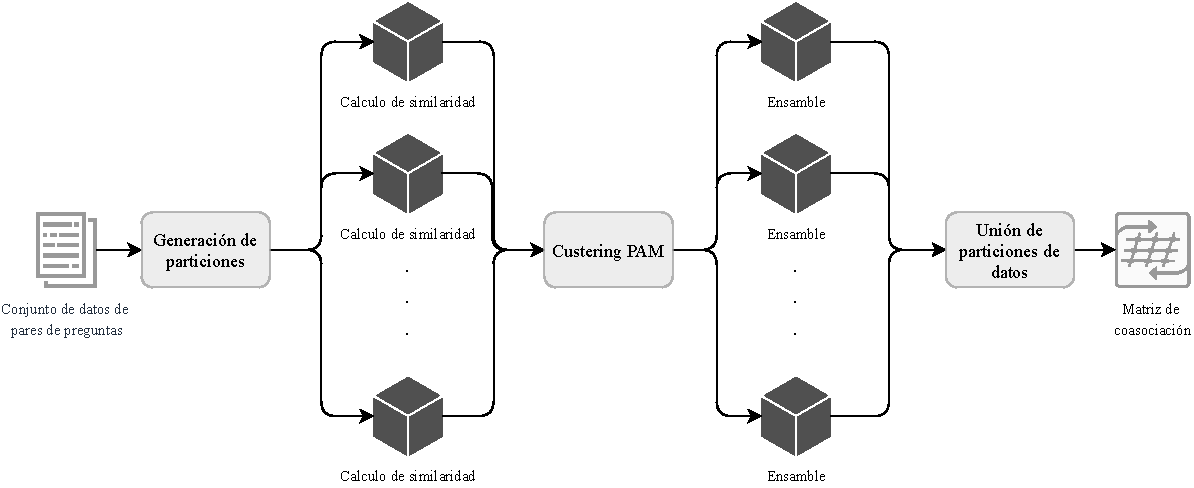
\includegraphics[width=1\linewidth]{8_problema_investigacion/imagenes/equal_distribuido}
	\caption{Infraestructura de la solución para generar una matriz de coasociación para un RS.}
	\label{fig:equaldistribuido}
\end{figure}

\bigskip Como se mencionó anteriormente, la generación de las matrices de distancia se realizarán de forma paralela, particionando el conjunto de datos de entrada y luego juntando los resultados para construir cada una de las matrices. Una vez que las matrices de similaridad son generadas en la memoria del nodo maestro se procederá a realizar el algoritmo de cluster en el mismo, paralelizando las distintas ejecuciones con el objetivo de optimizar los recursos de hardware y reducir el tiempo de ejecución. Las razones por la cual se eligió esta estrategia (en lugar de paralelizar la ejecuciones en todo el cluster de computadoras), son las siguientes:

\begin{itemize}
	\item Apache Spark no provee la funcionalidad de “replicar” un conjunto de datos y enviar tareas a un ejecutor en particular, para luego replicar el resultado. Es decir, si quisiéramos llevar a cabo el algoritmo de clustering en un nodo de datos en particular utilizando la matriz de similaridad completa y, al mismo tiempo, duplicar esta tarea tantas veces como ejecutores existan, podría optimizarse la utilización de recursos y aprovechar el paralelismo en cada uno de ellos. Por el momento, no existe una forma fácil y computacionalmente eficiente de realizar esta tarea, en una arquitectura basada en Hadoop.
	\item Evitar \textit{data-shuffling} excesivo entre entre nodos de datos. El data-shuffling es una operación que simplemente re-organiza y re-distribuye datos entre las particiones de datos apropiadas \citep{zhang2012optimizing}. Esto es un problema cuando se realiza de forma excesiva en un cluster de computadoras, provocando demasiada transferencia de datos entre cada uno de los nodos. Por ejemplo, antes de aplicar una función personalizada, en cuando se realiza shuffling puede ser necesario realizar un ordenamiento local en cada partición, re-particionar los datos en cada una de las computadoras para luego redistribuir las mismas dependiendo, por ejemplo, en una clave primaria. Dicho esto, queda en evidencia que este procedimiento conlleva un procesamiento de red y disco rígido (entrada/salida) que deriva en el incremento de tiempo de ejecución comparado con un ambiente que use una sola computadora y el intercambio de datos entre particiones se realice en la memoria local.
\end{itemize}

El algoritmo de clustering realizado en forma centralizada producirá como resultados archivos persistidos en el almacenamiento local que posibiliten aplicar un paralelismo basado en datos en el cuando el ensamble de clustering es aplicado. El formato de salida de cada una de las ejecuciones del algoritmo de clustering aplicado, posibilitarán que sea muy simple aplicar una función personalizada de ensamble de clustering distribuyendo los datos entre todas las particiones del cluster de computadoras y obteniendo una matriz de coasociación.

\subsubsection{Escalabilidad horizontal}
Es sabido que una computadora con una mejor configuración puede realizar más tareas que una con una configuración más débil, pero eso tiene una limitante. El costo de producir una computadora con buen rendimiento es alto, y no lo suficiente para justificar el costo. Por lo cual, la arquitectura elegida utiliza un cluster de computadoras para lograr un gran desempeño.

\bigskip Este tipo de sistemas escalan de una forma casi lineal con el número de servidores utilizados, y esto es posible debido al uso de particionamiento de datos \citep{pokorny2013nosql}. La distribución de datos horizontal posibilita dividir los cálculos computacionales en diferentes tareas concurrentes. Esto no es posible realizarlo fácilmente sin un algoritmo y una arquitectura que se adapte y sean pensados desde su concepción para este tipo de funcionalidad, tales como MapReduce y Hadoop.

\subsubsection{Escalabilidad y complejidad temporal}
En cuanto a la etapa de cálculo de similaridad para los distintos algoritmos tenidos en cuenta para el ensamble de clustering, siendo \(n\) el número de pares de preguntas de una muestra, y \(p = 2n\) el número de preguntas individuales. Al calcular la matriz triangular con entrada \(p\), tenemos:
\[\frac{p(p-1)}{2} = \frac{2n(2n-1)}{2} = 2n^2-n\]

Es decir, si el número de pares es \(n\), se realizarán \(2n^2-n\) cálculos por cada algoritmo de similaridad ejecutado. Además, si, por ejemplo, utilizamos \(\theta\) algoritmos de similaridad el número de cálculos de similaridad es aproximadamente \(\theta(2n2-n)\). Esto significa que al hacer cálculos de similaridad “todos contra todos” la complejidad temporal aumenta cuadráticamente, es decir \(O(n2)\)\footnote{La notación Big-O es el lenguaje y métrica que describe la eficiencia de un algoritmo. Simboliza una cota superior sobre el tiempo, basándose en una función en la cual la variable independiente puede cambiar dependiendo de la naturaleza del algoritmo (por ejemplo, tamaño de la estructura de datos o cantidad de iteraciones). \citep{cormen2009introduction}}\footnote{La notación Big-O tiende a eliminar constantes y términos no dominantes, ya que solo se centra en indicar cómo el algoritmo escala. }. Siendo estrictos, \(\theta(2n2-n)\). no sería apropiado, ya que cada uno de los diferentes algoritmos de similaridad tiene distinta complejidad interna y el tiempo varía entre cada uno de ellos, es por eso que la métrica de complejidad opta por eliminar constantes y multiplicadores a favor de la simplicidad.

\bigskip Al terminar el cálculo de similaridad, la arquitectura prevista procede a realizar un algoritmo de clustering con los resultados. Otra vez, siendo \(n\) el número de ítems (preguntas individuales), \(k\) el número de clusters elegido e \(i\) el número de iteraciones, para un tiempo \(t\) para calcular la distancia entre dos preguntas, tenemos una complejidad de \(O(n \cdot k \cdot i \cdot t)\), suponiendo que todas las iteraciones son realizadas y dejando de lado la etapa de optimización de medoides para el algoritmo PAM. Por otro lado, la arquitectura propone que el cálculo de distancia se ha realizado en una etapa anterior y las mismas son almacenadas en una estructura de datos en forma de \textit{tabla hash}\footnote{Una tabla hash es una estructura de datos que asocia claves con valores. La operación principal que soporta de manera eficiente es la búsqueda mediante una función hash.} en la cual es posible obtener la distancias de dos elementos haciendo una búsqueda indexada mediante una función hash precalculada, por lo cual, la complejidad temporal promedio en un escenario ideal será de \(O(1)\) (constante), y la complejidad final de la etapa de clustering de \(O(n \cdot k \cdot i)\), y para \(N\) ejecuciones, obtendremos \(O(N \cdot n \cdot k \cdot i)\).

\bigskip Por último, la etapa de ensamble de clustering utiliza la combinación de las \(n\) preguntas individuales en las \(N\) ejecuciones del algoritmo de clustering, obteniendo \(x = N \times n\) registros. Cada uno de esos registros son agrupados mediante una función \textit{group by}, una función que tiene una complejidad conocida de  \(O(x \cdot \log(x))\). El conjunto de datos generado es combinado con sí mismo para obtener las intersecciones, es decir \(O(x^2)\). Dado que el término \(x^2\) escala más rápido que el término \(x \cdot \log(x\)) es posible simplificar la complejidad temporal a solo \(O(x^2)\), o también \(O(N^2 \cdot n^2)\).

\bigskip De forma simplificada, la complejidad total que ofrece el método propuesto es de \(O(n^2 + Nnki + N^2n^2)\), lo cual es una función cuadrática que depende de la cantidad de preguntas individuales \(n\). Lo anterior, deja en evidencia la importancia de utilizar sistemas distribuidos y paralelismo basado en datos, ya que si bien la cantidad de cálculos total no cambia, seria posible hacer que el valor de \(n\) (y por lo tanto la cantidad de cálculos) que trabaja cada nodo de ejecución y cada ejecutor en cada uno de ellos sea más pequeño, según la cantidad de nodos o servidores de ejecución. En un contexto ideal y como modelo simplificado, por ejemplo, si se cuenta con un cluster de computadoras de \(8\) nodos y cada uno de ellos procesa \(n/8\) (\(n_{nuevo}=n / n\acute{u}mero\_de\_nodos\)) preguntas individuales, se realizarán \((n/8)^2=n^2/64\) cálculos de similaridad en cada uno de ellos, es decir, la cantidad de cálculos total, también se reducen de forma cuadrática. El ejemplo de la Figura \ref{fig:complejidad_temporal_figura}, es el modelo simplificado anteriormente mencionado, con fines didácticos que posee paralelismo de datos perfecto, cada uno de los nodos con la misma configuración y sin tener en cuenta tiempos de entrada/salida y re-particionamiento de datos. Se muestra la curva temporal de 4 clusters distintos de computadoras, con 1, 2, 4 y 8 nodos.

\begin{figure}[h!]
	\centering
	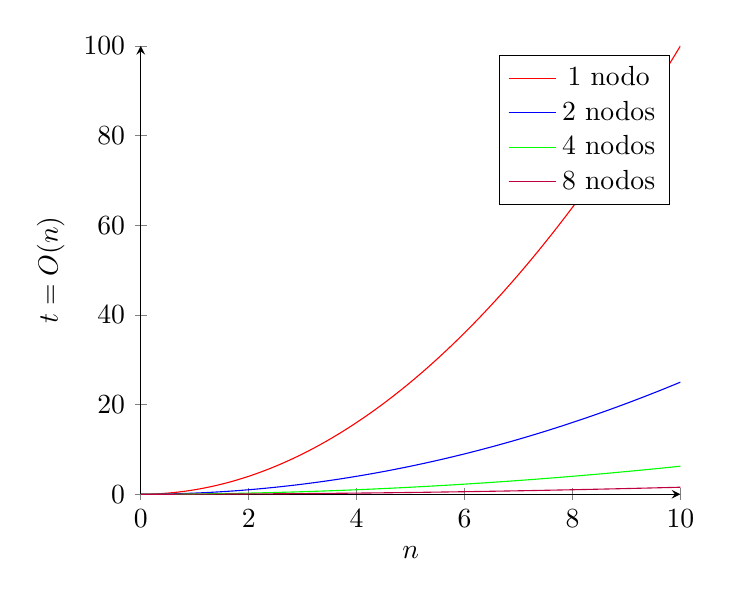
\begin{tikzpicture}
		\centering
		\begin{axis}[
			axis lines = left,
			xlabel = $n$,
			ylabel = {$t = O(n)$},
			]
			\addplot [domain=0:10, samples=100, color=red,] {x^2};
			\addlegendentry{1 nodo}

			\addplot [domain=0:10, samples=100, color=blue,]{x^2/4};
			\addlegendentry{2 nodos}

			\addplot [domain=0:10, samples=100, color=green,]{x^2/16};
			\addlegendentry{4 nodos}

			\addplot [domain=0:10, samples=100, color=purple,]{x^2/64};
			\addlegendentry{8 nodos}
		\end{axis}
	\end{tikzpicture}
	\caption{Aproximación de funciones de complejidad temporal según la cantidad de nodos del cluster de computadoras.}
	\label{fig:complejidad_temporal_figura}
\end{figure}

\bigskip La unidad básica de Apache Spark es llamada0 tarea, y la cantidad de tareas depende del número de particiones del conjunto de datos de entrada. Cada una de las tareas se encuentra en un hilo de ejecución de una JVM\footnote{Del inglés \textit{Java Virtual Machine}, es una máquina virtual que permite ejecutar programas en código intermedio Java.}, dedicado exclusivamente a un \textit{ejecutor}. Uno o más ejecutores son desplegados en los distintos \textit{nodos} del cluster de computadoras \citep{janardhanan2020optimum}. Es decir, que el paralelismo obtenido por la infraestructura Spark, depende de los tres niveles: tareas, ejecutores y nodos; así como también de la naturaleza del algoritmo que se ejecuta en la misma. Con el fin de dar un ejemplo aplicable al cálculo de similaridad, se configura un cluster de computadoras de 4 nodos, y 4 ejecutores en cada uno de ellos. Si cada uno de los ejecutores asigna 1-14 núcleos de CPU de forma dinámica, el número total de núcleos variará entre 4 y 56. Esto significa, que habrá de 4 a 56 tareas ejecutándose paralelamente en la infraestructura definida.
